\documentclass{article}
\usepackage{amsmath}
\usepackage{amssymb}
\usepackage{amsfonts}
\usepackage{geometry}
\usepackage{graphicx}
\usepackage[all]{xy}
\geometry{a4paper,scale=0.75}

\title{Solution for Exercise sheet 2}
\author{Yikai Teng, You Zhou}
\date{Exercise session: Thu. 8-10}

\begin{document}

\maketitle

\paragraph{Exercise 2.1}
\subparagraph{(a)}Let $\{S_n^2\}_{n\in\mathbb{Z}}$ be a sequence of spheres. Fix $x_n$ in each sphere $S_n^2$ and consider
\[Y:=\mathbb{R}\coprod\left(\coprod_{n\in\mathbb{Z}}S_n^{2}\right).\]
Then the universal cover, as shown in the question sheet, is
\[\widetilde{X}=Y/\sim.\]
The equivalence relation $\sim$ on $Y$ is defined as
\[\forall x,y\in Y, p\sim q\Leftrightarrow\exists n\in\mathbb{Z} \text{ s.t. } x=n, y=x_n\text{ or }x=x_n, y=n.\]
To describe the covering map $p\colon\widetilde{X}\rightarrow X,$ we will denote points in $S^1$ by $\{e^{i\theta}:\theta\in\mathbb{R}\}$ and points in every $S^2$ by $\{(x,y,z)\in\mathbb{R}^3:x^2+y^2+z^2=1\}.$ In particular, in $X$ we let $e^{-i\pi/2}$ and $(0,0,1)$ be identified and in $Y$ we let $(0,0,1)\in S_n^2$ be identified with $n\in\mathbb{R}.$ Then $p$ maps $\theta\in\mathbb{R}$ to $e^{2\pi i\theta}\in S^1,$ and $(x,y,z)\in S_n^2$ to the ``same'' point $(x,y,z)\in S^2.$ In particular, all $x_n$ are mapped to the ``intersection'' of $S^1$ and $S^2$ in $X.$

Next we compute the deck transformation group $G$ of $\widetilde{X}.$ Suppose $\varphi\in G$ and $\tilde{x}\in\widetilde{X}.$ Since $\varphi(\tilde{x})$ and $\tilde{x}$ are mapped by $p$ to the same point in $X,$ the only possible choices of $\varphi(\tilde{x})$ is
\[\begin{cases}
  \tilde{x}+n \text{ for some }n\in\mathbb{Z}, & \mbox{if } \tilde{x}\in\mathbb{R} \\
  (x,y,z)\in S_n^2\text{ for some }n\in\mathbb{Z}, & \mbox{if } \tilde{x}=(x,y,z)\in S_m^2\text{ for some }m.
\end{cases}\]
The continuity of $\varphi$ forces $\varphi$ to be a transformation by $n$ units, with $n$ some integer. This shows that $G\cong\mathbb{Z}.$

Finally, the covering space theory tells us that since $\widetilde{X}$ is simply-connected, we have $\pi_1(X,x_0)\cong G\cong\mathbb{Z}.$

\subparagraph{(b)}
Since the universal cover is simply connected, the Hurewicz theorem tells us that
\[\pi_2(\widetilde{X},\tilde{x_0})\cong H_2(\widetilde{X},\mathbb{Z}).\]
Since covering maps induces isomorphisms on $n$-th homotopy groups for every $n\geq2,$ it suffices to compute $H_2(\widetilde{X},\mathbb{Z}).$

Let $A$ and $B$ denote $\mathbb{R}$ and $\coprod_{n\in\mathbb{Z}}S_n^2,$ as subsets of $\widetilde{X},$ respectively. Then $A\cap B=\coprod_{n\in\mathbb{Z}}\{\text{point}\}.$ and the interiors of $A$ and $B$ covers $\widetilde{X}.$ By the Mayer-Vietoris sequence
\[\cdots\rightarrow H_2(A\cap B,\mathbb{Z})\rightarrow H_2(A,\mathbb{Z})\oplus H_2(B,\mathbb{Z})\rightarrow H_2(\widetilde{X},\mathbb{Z})\rightarrow H_1(A\cap B,\mathbb{Z})\rightarrow\cdots\]
we have $H_2(A,\mathbb{Z})\oplus H_2(B,\mathbb{Z})\cong H_2(\widetilde{X},\mathbb{Z}).$ Since $\mathbb{R}$ can be seen as a CW-complex with no $n$-cells for $n\geq2,$ we have $H_2(A,\mathbb{Z})=0.$ Thus
\[H_2(\widetilde{X},\mathbb{Z})\cong H_2\left(\coprod_{n\in\mathbb{Z}}S_n^2,\mathbb{Z}\right)\cong\bigoplus_{n\in\mathbb{Z}}\mathbb{Z}\]


\subparagraph{(c)}We first construct a basis for $\pi_2(\widetilde{X},x_0).$ Let $f_n\colon (I^2,\partial I^2)\rightarrow (\widetilde{X}, \tilde{x_0})$ be the map illustrated in figure \ref{2.1_1} below.
\begin{figure}[ht]
  \centering
  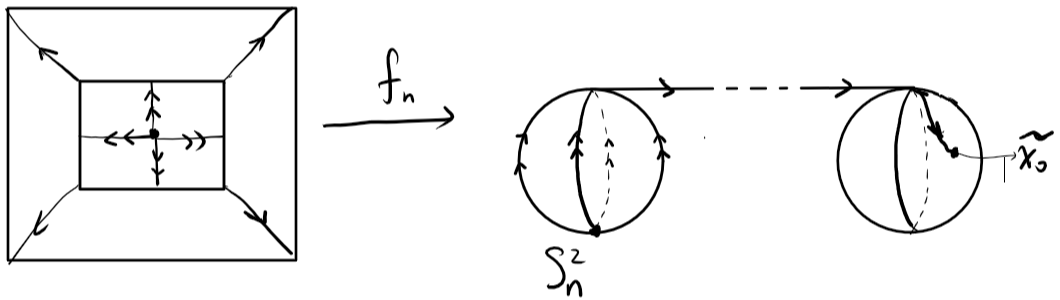
\includegraphics[width=13cm]{2.1_1.png}
  \caption{Definition of $f_n$}\label{2.1_1}
\end{figure}
So $f_n$ can be viewed as an element in $\pi_2(\widetilde{X},x_0).$ Addition of $f_n$ and $f_m$ and the fact that $f_n+f_m=f_m+f_n$ are illustrated in the picture below.
\begin{figure}[ht]
  \centering
  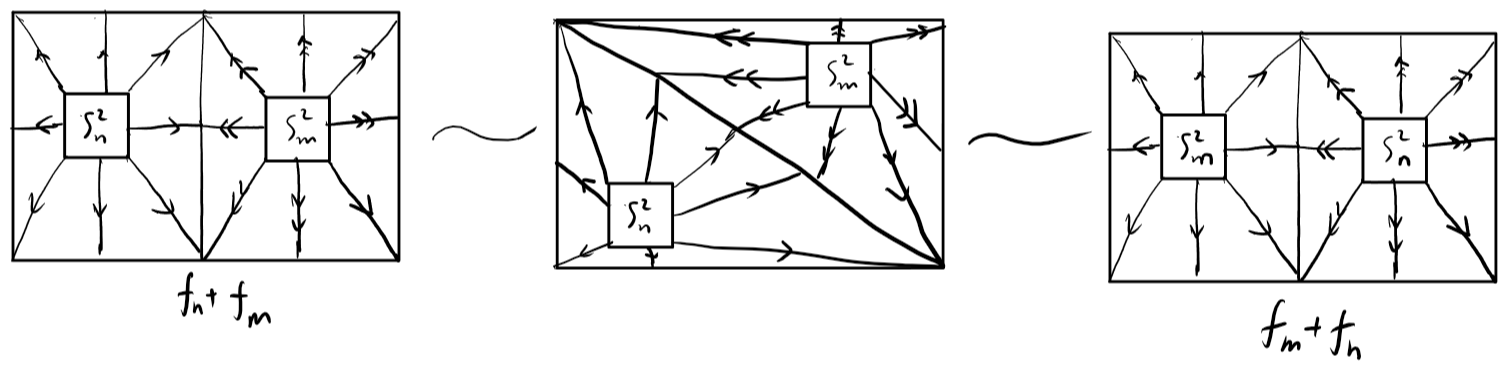
\includegraphics[width=13cm]{2.1_2.png}
  \caption{Commutativity of the addition}\label{2.1_2}
\end{figure}
We claim that $f_n$ and $f_m$ are not homotopy equivalent when $n\neq m$. Then we have an isomorphism
\[\pi_2(\widetilde{X},x_0)\xrightarrow{\cong} \bigoplus_{n\in\mathbb{Z}}\mathbb{Z}\]
that sends $f_n$ to $(\ldots,0,0,1,0,0,\ldots),$ where 1 is in the $n$-th position. Then $p\circ f_n$ is a basis of $\pi_2(X,x_0),$ where $p$ is the covering map described in part a.

Now we prove the claim above. Suppose not and let $H\colon I^2\times I\rightarrow \widetilde{X}$ be a continuous map such that $H(x,0)=f_n(x)$ and $H(x,1)=f_m(x).$ Then $H^{-1}(S_n^2)$ is a closed subset of $I^2\times I$ containing the
``inner square'' of the domain of $f_n$ (the smaller square drawn in figure \ref{2.1_1}). By continuity the boundary of $H^{-1}(S_n^2)$ must be mapped to the ``point of intersection'' of $S_n^2$ and the line $\mathbb{R},$ denoted by $y_n$ for short. For every $x\in S_n^2,$ the line $x\times[0,1]$ must have intersection with $\partial H^{-1}(S_n^2),$ i.e. there is some $t_x\in[0,1]$ such that $H(x,t_x)=y_n.$ But this would imply that $S^2$ can be retracted to a point, which is impossible. The idea is illustrated in figure \ref{2.1_3} below.

\begin{figure}[ht]
  \centering
  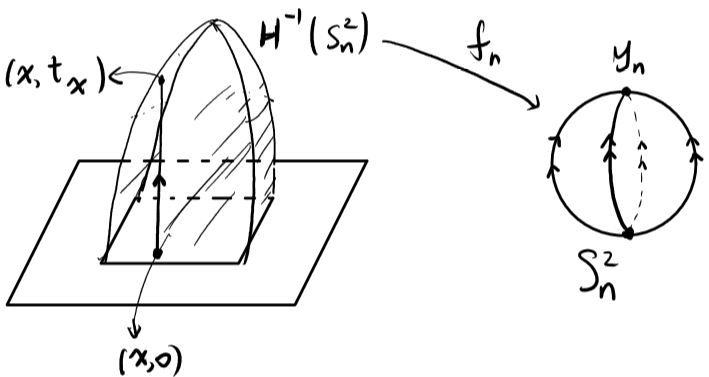
\includegraphics[width=6cm]{2.1_3.png}
  \caption{Study of $f_n$}\label{2.1_3}
\end{figure}


Finally, by the isomorphisms established above, describing the action of $\pi_1(X,x_0)$ on $\pi_2(X,x_0)$ is equivalent to describing the action of $\mathbb{Z}$ on $\bigoplus_{n\in\mathbb{Z}}\mathbb{Z}.$ The latter is not hard. It gives the required action to let $p\in\mathbb{Z}$ send $(\ldots,0,0,1,0,0,\ldots),$ where 1 is in the $n$-th position, to $(\ldots,0,0,1,0,0,\ldots),$ where 1 is in the $(n+p)$-th position.

\paragraph{Exercise 2.2}Let $\Sigma X$ denote the suspension of $X$ and denote by $x_1$ and $x_2$ the points $X\times\{0\}$ and $X\times\{1\}$ in $\Sigma X, $ respectively. Let
\[A:=\Sigma X\setminus \{x_1\}\text{ and }B:=\Sigma X\setminus \{x_2\},\]
then the interior of $A$ and $B$ covers $X.$ By Mayer-Vietoris sequence we have the exact sequence
\[\cdots\rightarrow \widetilde{H}_n(A\cap B)\rightarrow \widetilde{H}_n(A)\oplus \widetilde{H}_n(B)\rightarrow \widetilde{H}_n(\Sigma X)\rightarrow \widetilde{H}_{n-1}(A\cap B)\rightarrow\cdots\]
Note that both $A$ and $B$ are contractible and that $A\cap B$ and $X$ are homotopy equivalent. Thus all the reduced integral homology groups of $\Sigma X$ are trivial, which implies that $X$ is path-connected and that the $n$-th integral homology group of $\Sigma X$ is trivial for all $n\geq 1.$ So the Hurewicz theorem shows that $\pi_n(X,x_0)=0$ for all $n\geq1.$ Since $X$ is a CW-complex, Whitehead's theorem shows that $\Sigma X$ is contractible.

\paragraph{Exercise 2.3}

\end{document}
